\documentclass[lang=cn,11pt,a4paper,cite=authornum]{paper}

\title{计算机网络实验一:数据链路层滑动窗口协议的设计与实现\ 实验报告}
\author{毛子恒 \\ 2019211397 \and 庞仕泽 \\ 2019211509}
\institute{北京邮电大学\ 计算机学院}

\date{\zhtoday}


% 本文档命令
\usepackage{array}
\newcommand{\ccr}[1]{\makecell{{\color{#1}\rule{1cm}{1cm}}}}
\nocite{*}

\begin{document}

\maketitle

\section{实验内容和实验环境描述}

\subsection{实验内容}

利用所学数据链路层原理,自己设计一个滑动窗口协议,在仿真环境下编程实现有噪音信道环境下两站点之间无差错双工通信。信道模型为8000 bps全双工卫星信道,信道传播时延270毫秒,信道误码率为$10^{-5}$,信道提供字节流传输服务,网络层分组长度固定为256字节。

通过该实验,进一步巩固和深刻理解数据链路层误码检测的CRC校验技术,以及滑动窗口的工作机理。滑动窗口机制的两个主要目标:

\begin{enumerate}
    \item 实现有噪音信道环境下的无差错传输;
    \item 充分利用传输信道的带宽。
\end{enumerate}

在程序能够稳定运行并成功实现第一个目标之后,运行程序并检查在信道没有误码和存在误码两种情况下的信道利用率。为实现第二个目标,提高滑动窗口协议信道利用率,需要根据信道实际情况合理地为协议配置工作参数,包括滑动窗口的大小和重传定时器时限以及ACK搭载定时器的时限。这些参数的设计,需要充分理解滑动窗口协议的工作原理并利用所学的理论知识,经过认真的推算,计算出最优取值,并通过程序的运行进行验证。

\subsection{实验环境}

\begin{itemize}
    \item macOS Big Sur 11.2.3
    \item Visual Studio Code 1.55.0
    \item Apple clang version 12.0.0
    \item GNU make 3.81
\end{itemize}

\section{软件设计}

\subsection{数据结构}

\begin{code}
\begin{minted}{C}
typedef unsigned int seq_nr;
typedef unsigned char frame_kind;

typedef struct
{
    frame_kind kind;             // 帧的种类
    unsigned char ack;           // ACK序号:最后一个被成功接收的帧序号
    unsigned char seq;           // 帧序号
    unsigned char data[MAX_PKT]; // 数据
    unsigned char padding[4];    // CRC校验段
} Frame;                         // 帧,与物理层通信;seq,data,padding只在DATA类型帧中有效

typedef struct
{
    unsigned char data[MAX_PKT];
    size_t len;
} Packet; // 包,与网络层通信

static bool phl_ready = false;  // 物理层是否就绪
static Packet out_buf[NR_BUFS]; // 接收窗口
static Packet in_buf[NR_BUFS];  // 发送窗口
static bool arrived[NR_BUFS];   // 标记帧是否到达的bit map

// 以下是主程序中的变量

seq_nr ack_expected = 0;       // 期望收到ACK的帧序号,发送窗口的下界
seq_nr next_frame_to_send = 0; // 下一个发出的帧序号,发送窗口的上界+1
seq_nr frame_expected = 0;     // 期望收到的帧序号,接收窗口的下界
seq_nr too_far = NR_BUFS;      // 接收窗口的上界+1
int i;
Frame r;              // 接收到的帧
int len;              // 接收到的帧的长度
seq_nr nbuffered = 0; // 接收到的帧的数量
int event;
int arg; // 事件接收到的参数
\end{minted}
\end{code}

\subsection{模块结构}

\begin{code}
\begin{minted}{C}
// 判断在窗口中是否有a<=b<c
static bool between(seq_nr a, seq_nr b, seq_nr c);

// 添加校验段,发送DATA帧到物理层
static void put_frame(unsigned char *frame, int len);

// 根据不同类型构建帧、发送帧、处理计时器
static void send_dllayer_frame(frame_kind fk, seq_nr frame_nr, seq_nr frame_expected);
\end{minted}
\end{code}

模块间调用关系如\figref{fig:img2}。

\begin{figure}[htbp]
    
    \centering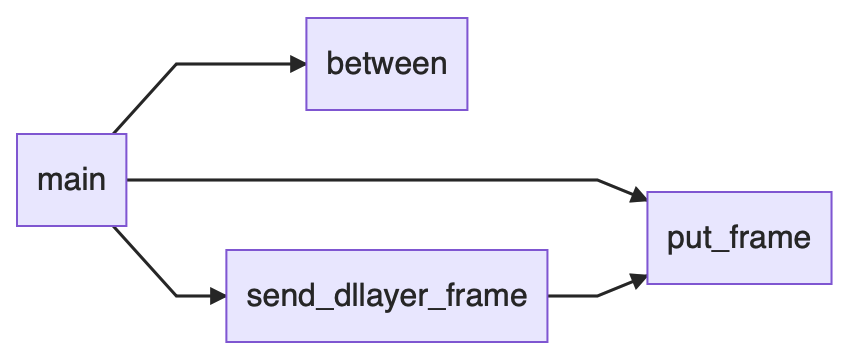
\includegraphics[width=0.4\textwidth]{./Images/img2.png}

    \caption{模块调用关系图\label{fig:img2}}

\end{figure}

\subsection{算法流程}

选择重传协议的算法流程如\figref{fig:img3}。

\begin{figure}[htbp]
    
    \centering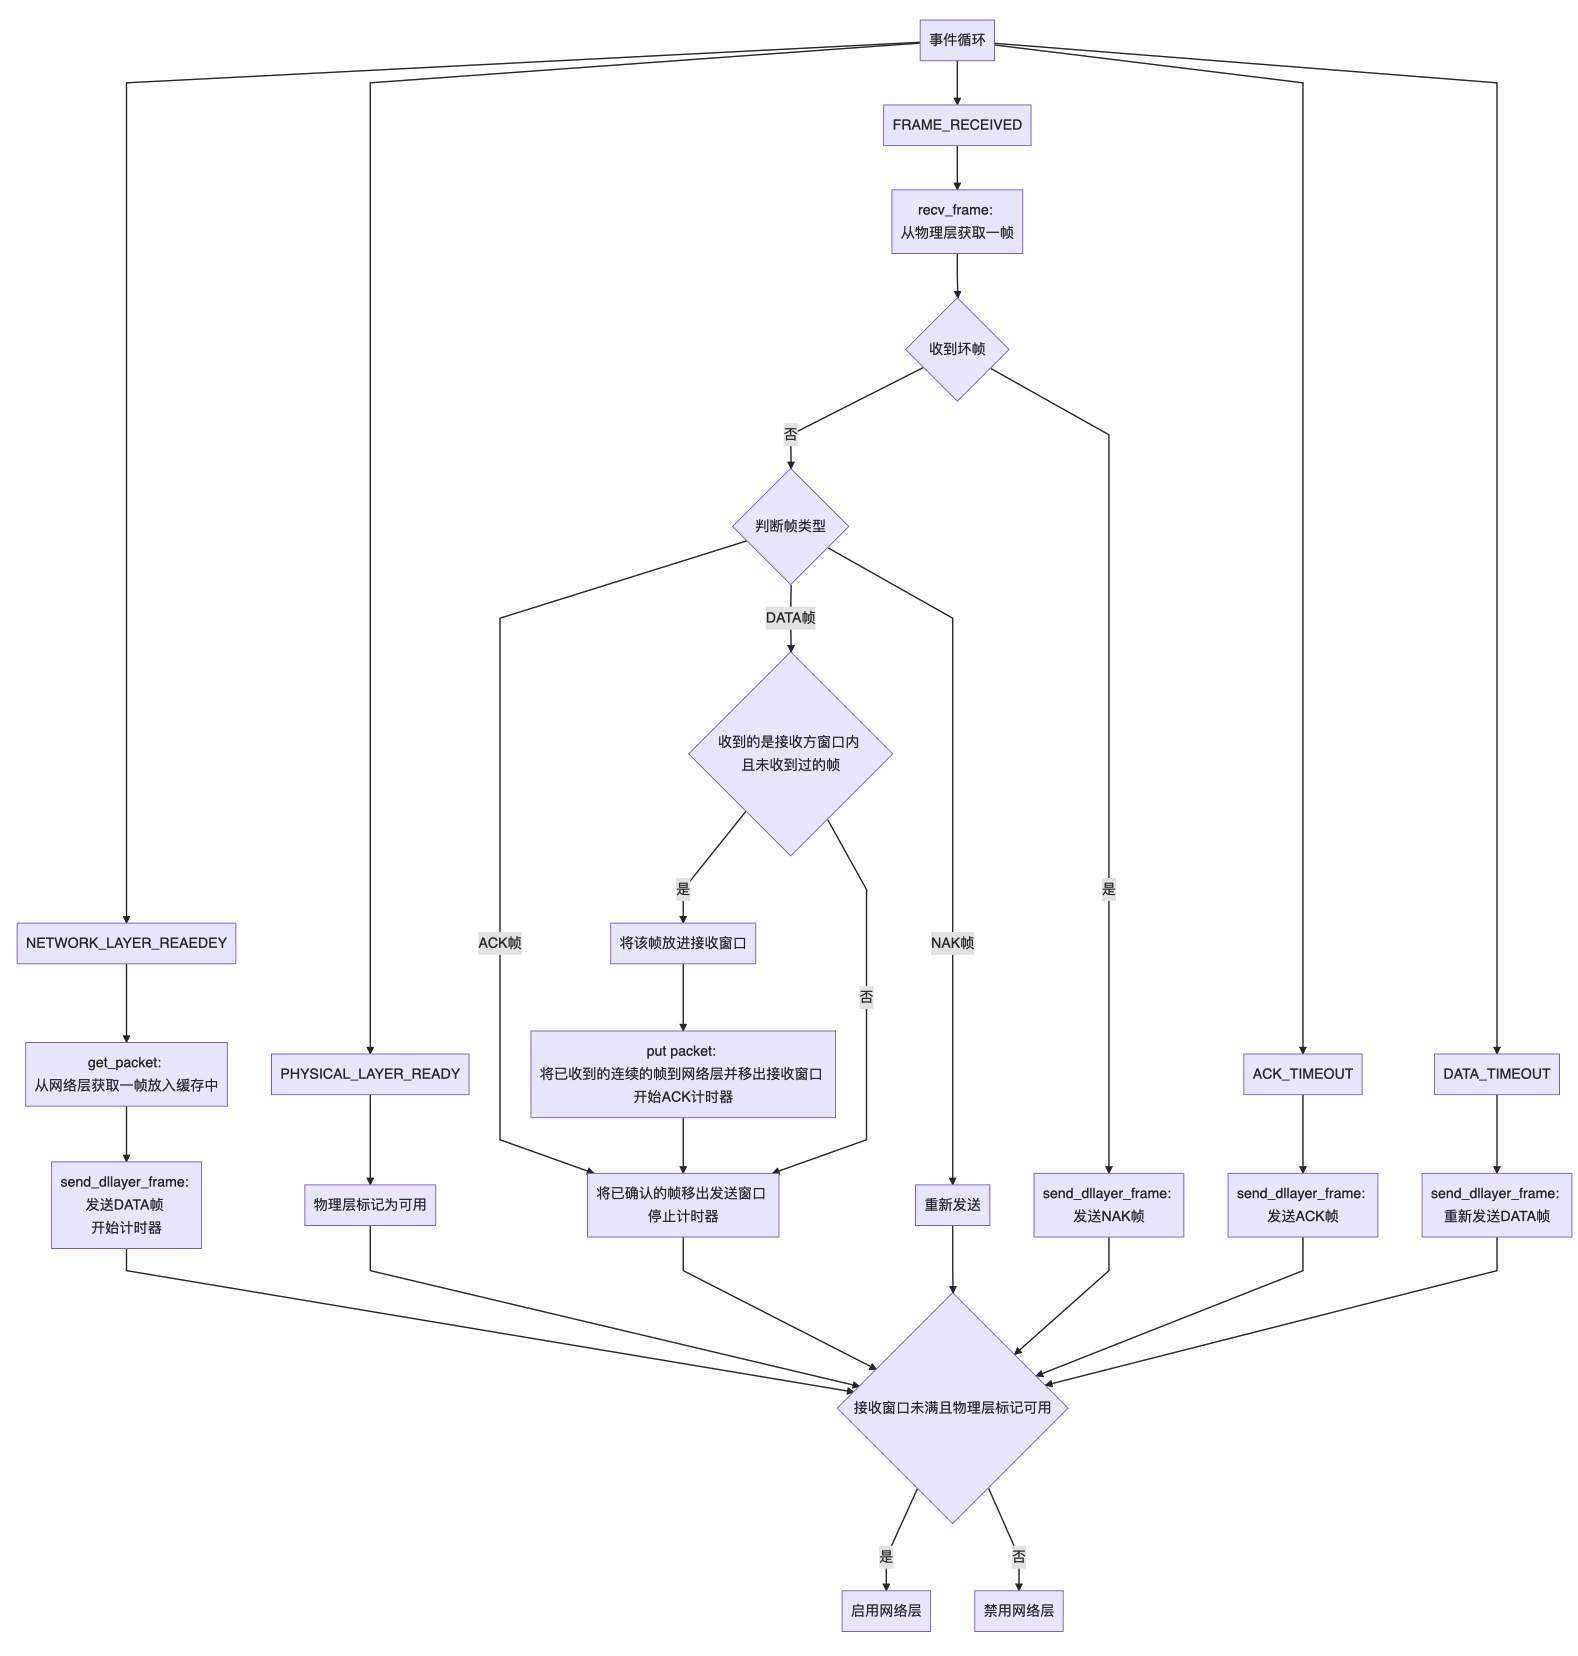
\includegraphics[width=\textwidth]{./Images/img3.png}

    \caption{算法流程图\label{fig:img3}}

\end{figure}

\section{实验结果分析}

\subsection{程序正确性和健壮性分析}

程序实现了在有误码信道环境中的无差错传输功能。在误码率较高的情况下仍然能够稳定运行超过1小时并且保持可观的信道利用率,可见程序健壮性较好。

\subsection{参数选择}

\subsubsection{窗口大小选择}

在无差错信道的情况下,窗口大小$W$应当满足以下表达式:

$$
    \left\{
    \begin{aligned}
         & t_p = 270\ ms                       \\
         & t_f = \frac{263*8}{8000}\times 1000\ ms        \\
         & \frac{W\cdot t_f}{2t_f+2t_p} \geq 1
    \end{aligned}
    \right.
$$

计算出$W\geq 4.05$。

当误码率较高时,取帧错误的概率$P=0.2$:

$$
    \left\{
    \begin{aligned}
         & t_p = 270\ ms                       \\
         & t_f = \frac{263*8}{8000}\times 1000\ ms        \\
         & \frac{W(1-P)\cdot t_f}{2t_f+2t_p} \geq 1
    \end{aligned}
    \right.
$$

计算出$W\geq 5.06$。因此,当误码率较高时,至少会用到6个发送窗口。

通过在程序运行时打印发送方窗口大小,我们发现在一定概率下会用到16个以上的发送窗口,因此,为了最大化信道利用率,把窗口大小设为32,$MAX\_SEQ$为63。

\subsubsection{超时参数选择}

数据帧超时参数$T_{data}$和ACK帧超时参数$T_{ack}$应当满足以下条件:

$$
    \left\{
    \begin{aligned}
         & T_{data} \geq T_{ack} + 2t_p + 2t_f \\
         & W\cdot t_f \geq T_{ack}            \\
    \end{aligned}
    \right.
$$

由于协议设计时不考虑整个包丢失的情况,所以理论上选择重传协议的$T_{data}$可以设计的很大,而$T_{ack}$需要有下限,否则协议效率会变低,$T_{ack}$的上限需要满足如上两个不等式,保证不会因为$T_{ack}$过长而导致发送方DATA计时器超时,同时保证不会因为$T_{ack}$过长而使得发送窗口满。

经实际测试,取回退N协议的$T_{ack}=280\ ms,T_{data}=1000$\ ms,选择重传协议的$T_{ack}=280\ ms,T_{data}=5000$\ ms。

\subsection{理论分析}

由于ACK帧和NAK帧长度很短,占比极小,所以假设这些帧能100\%传输。设当前信道误码率为$p$,每个帧长为263字节,一次发送成功的概率为:

$$
    P=(1-p)^{263\times 8} = (1-p)^{2102}
$$

假设一帧传输需要的次数为随机变量$X$,则其期望为:

$$
    E(X) = \sum_{i=1}^{\infty}i\cdot (1-P)^{i-1}\cdot P=\frac 1P
$$

因此理论最大信道利用率为:

$$
    \eta = \frac {256}{263\cdot E(x)}
$$

代入$p=0$,得:

$$\eta \approx 97.33\%$$

代入$p=10^{-5}$,得:

$$\eta \approx 95.31\%$$

代入$p=10^{-4}$,得:

$$\eta \approx 78.88\%$$

\subsection{测试结果分析}

回退N协议的测试结果见\tabref{tab:gbnresult}。

\begin{table}[!htbp]
    \centering
    \caption{回退N协议\ 性能测试记录表\label{tab:gbnresult}}
    \begin{tabular}{|c|c|c|c|c|c|c|}
        \hline
        \multirowcell{2}{序                                                           \\号} & \multirowcell{2}{命令} & \multirowcell{2}{说明} & \multirowcell{2}{运行时间 \\ (秒)} & \multicolumn{2}{c|}{\makecell[c]{接收方线路\\利用率(\%)}} & \multirowcell{2}{存在的问题} \\
        \cline{5-6}
          &                                                           &  &  & A & B & \\
        \hline
        1 & \makecell[l]{\mintinline{shell}{datalink -u A}                            \\ \mintinline{shell}{datalink -u B}} & 无误码信道数据传输 & 1247 & 53.26 & 96.97 & \\
        \hline
        2 & \makecell[l]{\mintinline{shell}{datalink A}                               \\ \mintinline{shell}{datalink B}} & \makecell[l]{站点A分组层平缓方式\\发出数据,站点B周期\\性交替“发送100秒,慢\\发100秒”} & 1219 & 40.27 & 75.15 &  \makecell[l]{与理论性能\\差距较大} \\
        \hline
        3 & \makecell[l]{\mintinline{shell}{datalink -u -f A}                         \\ \mintinline{shell}{datalink -u -f B}} & \makecell[l]{无误码信道,站点A和\\站点B的分组层都洪水\\式产生分组} & 1200 & 96.97 & 96.97 & \\
        \hline
        4 & \makecell[l]{\mintinline{shell}{datalink -f A}                            \\ \mintinline{shell}{datalink -f B}} & \makecell[l]{站点A/B的分组层都洪\\水式产生分组} & 1201 & 77.40 & 77.80 &  \makecell[l]{与理论性能\\差距较大} \\
        \hline
        5 & \makecell[l]{\mintinline{shell}{datalink -f --ber 1e-4 A}                 \\ \mintinline{shell}{datalink -f --ber 1e-4 B}} & \makecell[l]{站点 A/B 的分组层都洪\\水式产生分组,线路误\\码率设为$10^{-4}$} & 1311 & 31.86 & 32.48 & \makecell[l]{与理论性能\\差距较大} \\
        \hline
    \end{tabular}
\end{table}

选择重传协议的测试结果见\tabref{tab:result}。

\begin{table}[!htbp]
    \centering
    \caption{选择重传协议\ 性能测试记录表\label{tab:result}}
    \begin{tabular}{|c|c|c|c|c|c|c|}
        \hline
        \multirowcell{2}{序                                                           \\号} & \multirowcell{2}{命令} & \multirowcell{2}{说明} & \multirowcell{2}{运行时间 \\ (秒)} & \multicolumn{2}{c|}{\makecell[c]{接收方线路\\利用率(\%)}} & \multirowcell{2}{存在的问题} \\
        \cline{5-6}
          &                                                           &  &  & A & B & \\
        \hline
        1 & \makecell[l]{\mintinline{shell}{datalink -u A}                            \\ \mintinline{shell}{datalink -u B}} & 无误码信道数据传输 & 1268 & 54.00 & 96.97 & \\
        \hline
        2 & \makecell[l]{\mintinline{shell}{datalink A}                               \\ \mintinline{shell}{datalink B}} & \makecell[l]{站点A分组层平缓方式\\发出数据,站点B周期\\性交替“发送100秒,慢\\发100秒”} & 1201 & 52.74 & 95.37 & \\
        \hline
        3 & \makecell[l]{\mintinline{shell}{datalink -u -f A}                         \\ \mintinline{shell}{datalink -u -f B}} & \makecell[l]{无误码信道,站点A和\\站点B的分组层都洪水\\式产生分组} & 1234 & 96.97 & 96.97 & \\
        \hline
        4 & \makecell[l]{\mintinline{shell}{datalink -f A}                            \\ \mintinline{shell}{datalink -f B}} & \makecell[l]{站点A/B的分组层都洪\\水式产生分组} & 1600 & 94.92 & 94.52 & \\
        \hline
        5 & \makecell[l]{\mintinline{shell}{datalink -f --ber 1e-4 A}                 \\ \mintinline{shell}{datalink -f --ber 1e-4 B}} & \makecell[l]{站点 A/B 的分组层都洪\\水式产生分组,线路误\\码率设为$10^{-4}$} & 1225 & 56.67 & 59.63 & \makecell[l]{与理论性能\\差距较大} \\
        \hline
    \end{tabular}
\end{table}

\subsection{实验结果分析}

回退N协议与理论性能差距较大,仅与选择重传协议的性能作对比参考。

观察选择重传协议第五组测试的日志,发现其中经常出现类似\figref{fig:img1}的情况。

\begin{figure}[htbp]

    \centering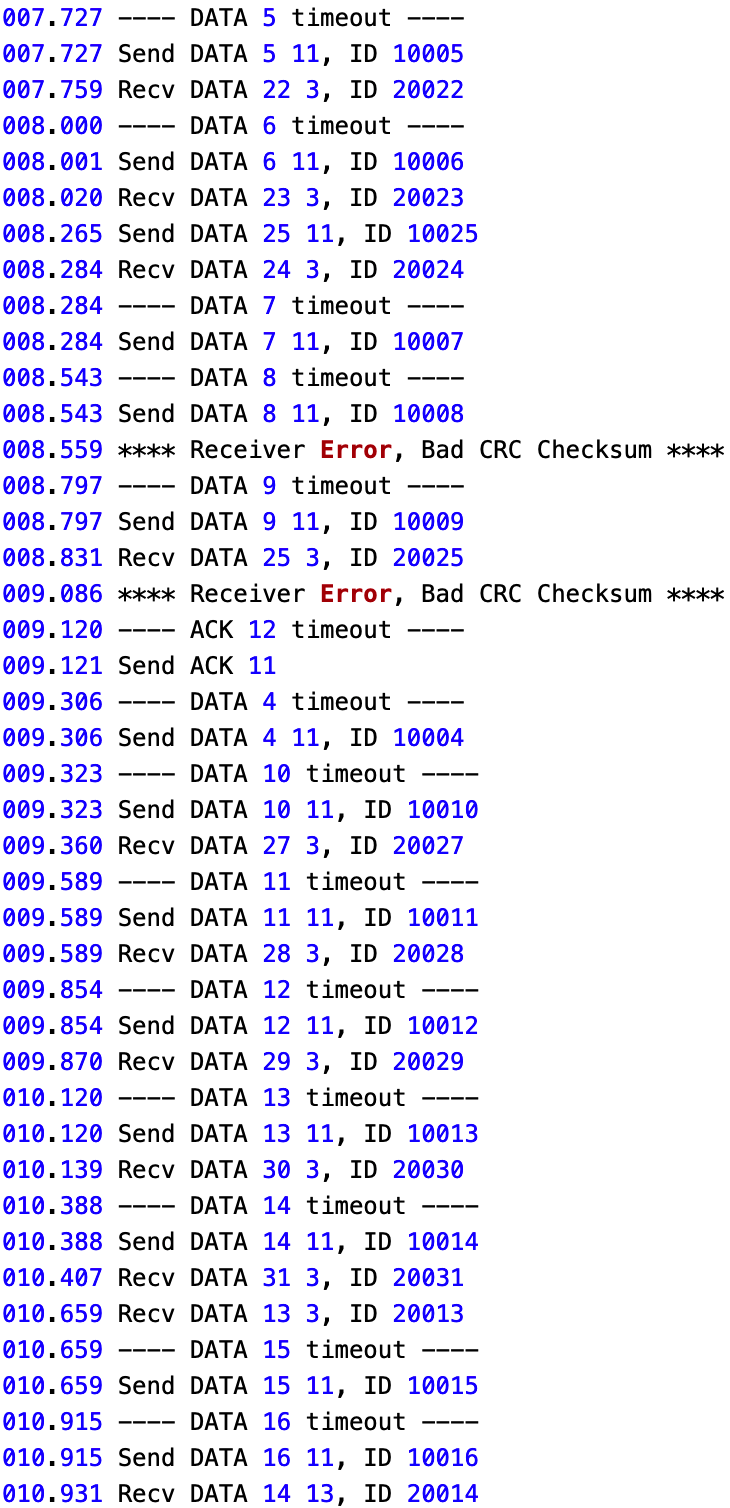
\includegraphics[width=0.4\textwidth]{./Images/img1.png}

    \caption{常见的导致信道利用率低的情况\label{fig:img1}}

\end{figure}

在第五组测试中,误码率为$p=10^{-4}$,每个帧发送失败的概率为$1-(1-p)^{2102}=0.19$,在一个窗口内平均有6个发送失败的帧。

在发生多次错误时,选择重传协议只会对第一个发送失败的帧发送NAK,当发送方重发该帧时,再发第二个失败的帧的NAK,此时会有大量收到但未确认的帧积压在接收方的缓冲区内,导致这些帧在发送方超时,因而产生大量不必要的重传。

我认为解决方法有两个:其一是弃用累计确认,对每个帧单独确认;其二是对每个错帧都单独发送NAK,取消每次只有一个NAK帧的限制。

我实现了较容易的第二种方案。具体来说,将NAK帧的\mintinline{C}{ack}字段含义改变为:否认某一个编号的帧并要求重发,同时取消\mintinline{C}{no_nak}变量。

改进后的选择重传协议的性能测试结果记录如\tabref{tab:result2}。可见第五组测试的性能得到大幅度提高。

\begin{table}[!htbp]
    \centering
    \caption{改进后的选择重传协议\ 性能测试记录表\label{tab:result2}}
    \begin{tabular}{|c|c|c|c|c|c|c|}
        \hline
        \multirowcell{2}{序                                                           \\号} & \multirowcell{2}{命令} & \multirowcell{2}{说明} & \multirowcell{2}{运行时间 \\ (秒)} & \multicolumn{2}{c|}{\makecell[c]{接收方线路\\利用率(\%)}} & \multirowcell{2}{存在的问题} \\
        \cline{5-6}
          &                                                           &  &  & A & B & \\
        \hline
        1 & \makecell[l]{\mintinline{shell}{datalink -u A}                            \\ \mintinline{shell}{datalink -u B}} & 无误码信道数据传输 & 1282 & 54.43 & 96.97 & \\
        \hline
        2 & \makecell[l]{\mintinline{shell}{datalink A}                               \\ \mintinline{shell}{datalink B}} & \makecell[l]{站点A分组层平缓方式\\发出数据,站点B周期\\性交替“发送100秒,慢\\发100秒”} & 1296 & 53.91 & 95.04 & \\
        \hline
        3 & \makecell[l]{\mintinline{shell}{datalink -u -f A}                         \\ \mintinline{shell}{datalink -u -f B}} & \makecell[l]{无误码信道,站点A和\\站点B的分组层都洪水\\式产生分组} & 1261 & 96.97 & 96.97 & \\
        \hline
        4 & \makecell[l]{\mintinline{shell}{datalink -f A}                            \\ \mintinline{shell}{datalink -f B}} & \makecell[l]{站点A/B的分组层都洪\\水式产生分组} & 1603 & 94.99 & 95.15 & \\
        \hline
        5 & \makecell[l]{\mintinline{shell}{datalink -f --ber 1e-4 A}                 \\ \mintinline{shell}{datalink -f --ber 1e-4 B}} & \makecell[l]{站点 A/B 的分组层都洪\\水式产生分组,线路误\\码率设为$10^{-4}$} & 3603 & 79.11 & 79.40 & \\
        \hline
    \end{tabular}
\end{table}

\subsection{存在的问题}

经过改进后的选择重传协议在部分情况下仍然与理论情况存在细微差距,我推测和程序本身的延迟,以及我们在计算时没有考虑ACK和NAK帧有关,此外计时器参数仍然可以进行细微的调整,以便适应不同误码率的情况。

\section{研究与探索的问题}

\subsection{CRC校验能力}

本次实验采用32位CRC校验码,理论上可以检测出所有影响到奇数位的错误和所有长度小于等于32的突发错误。

因此,只有发生33位以上的突发错误,坏帧才有可能通过检测。设一帧中出现突发错误的位数为随机变量$X$,则可以认为$X$满足泊松分布即$X\sim \pi(\lambda)$,其中$\lambda = np_n = 2104\times 10^{-5} = 2.104\times 10^{-2}$,此时:

$$
    P\{33\leq X\leq 2104\} = \sum_{k=33}^{2104} \frac{\lambda^k e^{-\lambda}}{k!} \approx 5.163\times 10^{-93}
$$

而这样的坏帧通过检测的概率为$2^{-32}$,因此检测不出坏帧的概率为:

$$
    P = 2^{-32}\cdot P\{33\leq X\leq 2104\}\approx 1.202\times 10^{-102}
$$

理想情况下客户每天发送帧的个数为:

$$
    k = \frac{95.31\%\times 8000\times 60\times 60\times 24}{263\times 8}\times 50\% \approx 156554
$$

因此理论上发生一次误码需要$\frac 1{365\cdot k\cdot P}\approx 1.455\times 10^{94}$年。

此外,即使在本层出现没有检测到的错误,理论上上层协议也会有检错和纠错措施,能对本层漏检的错误进行补偿。

\subsection{CRC校验和的计算方法}

查表法和手算CRC校验和是等效的,手算CRC校验和时是根据当前被除数最高位1或0判断是否异或$G(x)$,然而查表法先预处理8位除以$G(x)$的余数,之后每次除法从从表中取最高字节的余数,和原来余数的低24位异或得到新的余数。

值得注意的是这里的查表法默认是最低有效位在前。我实现的构造查表数组算法如下:

\begin{code}
\begin{minted}{C}
    void make_crc32_table(unsigned int crc_table[])
    {
        for(int i=0; i<256; i++)
        {
            unsigned int value = i;
            for(int j=0; j<8; j++)
            {
                if(value&1)
                    value = (value >> 1) ^ 0xedb88320;
                else
                    value = (value >> 1);
            }
            crc_table[i] = value;
        }
    }
\end{minted}
\end{code}

\subsection{程序设计方面的问题}

跟踪功能主要是便于调试,在程序出错时能快速定位出错位置,或者实时观察某些变量的取值以便针对性地进行性能优化。我的程序中多次调用了跟踪函数,并且将其应用到调试中。

\mintinline{C}{get_ms()}函数可以调用\mintinline{C}{time.h}中的\mintinline{C}{clock()}函数实现,具体来说,在进入主函数的\mintinline{C}{while}循环前调用该函数获取初始时间,之后每次调用\mintinline{C}{get_ms()}函数时获取当前时间并且减去初始时间。

\mintinline{C}{lprintf}函数使用可变参数实现,原型为\mintinline{C}{int lprintf(const char *format,...)},通过\mintinline{C}{format}字符串获取输出格式,之后用\mintinline{C}{va_list}获取之后的参数,传入\mintinline{C}{__v_lprintf}函数,根据格式输出。

DATA帧计时器需要和帧一一对应,当计时器超时时需要重发该计时器对应的帧,此后计时器需要清零。而ACK计时器关注的是第一个被成功接收但是没有发出ACK的帧,因此调用\mintinline{C}{start_ack_timer}后不会被清零,当发送ACK进行累计确认后才清零。

\subsection{软件测试方面的问题}

\begin{itemize}
    \item 无误码信道,主要考察协议数据包的设计,如果冗余信息较少则可以取得较高的信道利用率。
    \item 交替发送、停发,主要考察计时器参数的设计,较好的参数能够保证在各种情况下都能防止窗口满并且避免冗余重传。
    \item 洪水模式,考察协议的ACK、NAK帧的设计和流量控制能力,如果协议的流量控制系统较弱,或者ACK、NAK帧的发送时机不恰当,协议容易发生死锁。
    \item 高误码率模式,考察协议重传效率,如果协议在高误码率时有多次冗余的重传,则信道利用率会降低。
\end{itemize}

\subsection{对等协议实体之间的流量控制}

通过有限的发送方和接收方窗口实现流量控制。当发送方窗口满时,将调用\mintinline{C}{disable_network_layer()}来禁止网络层发来数据包。而当接收方窗口满时将会拒绝发送来的帧,引发发送方超时重传。

\subsection{与标准协议的对比}

本协议设计时只考虑到了延迟固定、包大小固定、误码率固定、带宽固定的情况,而在实际应用中这些量都有可能发生变化,协议需要一个自适应机制来应对不同的情况,例如通过拆分数据包使其变成小帧从而降低重发的频率、在不同误码率和延迟时自动调整计时器参数等。

\section{实验总结和心得体会}

本次程序的编码和调试大约花费我5个小时的时间,期间代码实现大部分参考了教材中的程序和实验材料中的示例。

在实现期间,由于对C语言和协议本身理解不够深刻,将\mintinline{C}{#define inc(k) k = (k + 1) & MAX_SEQ}误写作\mintinline{C}{#define inc(k) k = (k + 1) % MAX_SEQ},导致程序运行时会出现窗口过长而出现错误,经过几十分钟的调试才发现帧的编号出现问题。

由于事先配置好环境,对C语言语法本身也较为熟悉,并且实现之前认真阅读了课本内容和库文档,在这些部分没有遇到太多问题。

在测试时我发现程序在误码率较高时效率低下,通过查看日志分析原因,进而提出了改进的方法,使得程序在高误码率的情况下得到了可观的效率。

经过本次实验,我对选择重传协议有了更深刻的理解,另外对于协议的不足之处也有了认识,这是只看课本学习不到的知识。此外,通过阅读库代码和上手实践,我对事件驱动的网络编程有了大体的观念,这对于实践课实现DNS中继服务器有很大的帮助。在阅读代码的过程中,我也留意了编码规范和格式等一些细节,对我以后的C语言编程也会有很大帮助。

\newpage

\appendix

\section{源程序}

\begin{code}
\caption{datalink.c}
\begin{minted}{C}
    #include <stdio.h>
    #include <string.h>
    #include <stdbool.h>
    
    #include "protocol.h"
    #include "datalink.h"
    
    #define MAX_PKT 256
    #define MAX_SEQ 63
    #define NR_BUFS ((MAX_SEQ + 1) / 2)
    #define DATA_MAX_TIME 5000
    #define ACK_MAX_TIME 280
    
    #define inc(k) k = (k + 1) & MAX_SEQ
    
    typedef unsigned int seq_nr;
    typedef unsigned char frame_kind;
    
    typedef struct
    {
        frame_kind kind;             // 帧的种类
        unsigned char ack;           // ACK序号:最后一个被成功接收的帧序号
        unsigned char seq;           // 帧序号
        unsigned char data[MAX_PKT]; // 数据
        unsigned char padding[4];    // CRC校验段
    } Frame;                         // 帧,与物理层通信;seq,data,padding只在DATA类型帧中有效
    
    typedef struct
    {
        unsigned char data[MAX_PKT];
        size_t len;
    } Packet; // 包,与网络层通信
    
    static bool phl_ready = false;  // 物理层是否就绪
    static Packet out_buf[NR_BUFS]; // 接收窗口
    static Packet in_buf[NR_BUFS];  // 发送窗口
    static bool arrived[NR_BUFS];   // 标记帧是否到达的bit map
    
    // 判断在窗口中是否有a<=b<c
    static bool between(seq_nr a, seq_nr b, seq_nr c)
    {
        return a <= b && b < c || c < a && a <= b || b < c && c < a;
    }
    
    // 添加校验段,发送DATA帧到物理层
    static void put_frame(unsigned char *frame, int len)
    {
        *(unsigned int *)(frame + len) = crc32(frame, len);
        send_frame(frame, len + 4);
        phl_ready = false;
    }
    
    // 根据不同类型构建帧、发送帧、处理计时器
    static void send_dllayer_frame(frame_kind fk, seq_nr frame_nr, seq_nr frame_expected)
    {
        Frame s;
        s.kind = fk;
        s.ack = (frame_expected + MAX_SEQ) % (MAX_SEQ + 1);
        if (fk == FRAME_DATA)
        {
            s.seq = frame_nr;
            memcpy(s.data, out_buf[frame_nr % NR_BUFS].data, out_buf[frame_nr % NR_BUFS].len);
            dbg_frame("Send DATA %d %d, ID %d\n", s.seq, s.ack, *(short *)s.data);
            put_frame((unsigned char *)&s, 3 + out_buf[frame_nr % NR_BUFS].len);
            start_timer(frame_nr % NR_BUFS, DATA_MAX_TIME);
        }
        else
        {
            if (fk == FRAME_NAK)
            {
                s.ack = frame_expected;
                dbg_frame("Send NAK %d\n", frame_expected);
            }
            else
                dbg_frame("Send ACK %d\n", s.ack);
            send_frame((unsigned char *)&s, 3);
        }
        stop_ack_timer();
    }
    
    int main(int argc, char **argv)
    {
        seq_nr ack_expected = 0;       // 期望收到ACK的帧序号,发送窗口的下界
        seq_nr next_frame_to_send = 0; // 下一个发出的帧序号,发送窗口的上界+1
        seq_nr frame_expected = 0;     // 期望收到的帧序号,接收窗口的下界
        seq_nr too_far = NR_BUFS;      // 接收窗口的上界+1
        int i;
        Frame r;              // 接收到的帧
        int len;              // 接收到的帧的长度
        seq_nr nbuffered = 0; // 接收到的帧的数量
        int event;
        int arg; // 事件接收到的参数
    
        protocol_init(argc, argv);
        lprintf("Designed by xqmmcqs, build: " __DATE__ "  "__TIME__
                "\n");
    
        disable_network_layer();
    
        while (true)
        {
            event = wait_for_event(&arg);
            // lprintf("NBUFFERED %d ACK_EXPECTED %d NEXT_FRAME_TO_SEND %d\n", nbuffered, ack_expected, next_frame_to_send);
    
            switch (event)
            {
            case NETWORK_LAYER_READY: // 网络层就绪
                nbuffered++;
                out_buf[next_frame_to_send % NR_BUFS].len = get_packet(out_buf[next_frame_to_send % NR_BUFS].data);
                send_dllayer_frame(FRAME_DATA, next_frame_to_send, frame_expected); // 发送DATA帧
                inc(next_frame_to_send);
                break;
    
            case PHYSICAL_LAYER_READY:
                phl_ready = 1;
                break;
    
            case FRAME_RECEIVED:
                len = recv_frame((unsigned char *)&r, sizeof r);
                if (len < 5 && len != 3)
                    break;
                if (len >= 5 && crc32((unsigned char *)&r, len) != 0) // 校验错误
                {
                    dbg_event("**** Receiver Error, Bad CRC Checksum ****\n");
                    send_dllayer_frame(FRAME_NAK, 0, r.seq);
                    break;
                }
    
                if (r.kind == FRAME_ACK)
                    dbg_frame("Recv ACK %d\n", r.ack);
    
                if (r.kind == FRAME_DATA)
                {
                    dbg_frame("Recv DATA %d %d, ID %d\n", r.seq, r.ack, *(short *)r.data);
                    start_ack_timer(ACK_MAX_TIME);
                    if (between(frame_expected, r.seq, too_far) && !arrived[r.seq % NR_BUFS])
                    {
                        arrived[r.seq % NR_BUFS] = true;
                        memcpy(in_buf[r.seq % NR_BUFS].data, r.data, len - 7);
                        in_buf[r.seq % NR_BUFS].len = len - 7;
                        while (arrived[frame_expected % NR_BUFS]) // 将接收缓冲区中连续的已收到的帧发送到网络层
                        {
                            put_packet(in_buf[frame_expected % NR_BUFS].data, in_buf[frame_expected % NR_BUFS].len);
                            arrived[frame_expected % NR_BUFS] = false;
                            inc(frame_expected);
                            inc(too_far);
                            start_ack_timer(ACK_MAX_TIME);
                        }
                    }
                }
    
                if (r.kind == FRAME_NAK && between(ack_expected, r.ack, next_frame_to_send)) // 发送特定的NAK帧
                {
                    dbg_frame("Recv NAK %d\n", r.ack);
                    send_dllayer_frame(FRAME_DATA, r.ack, frame_expected);
                    break;
                }
    
                while (between(ack_expected, r.ack, next_frame_to_send)) // 累计确认
                {
                    nbuffered--;
                    stop_timer(ack_expected % NR_BUFS);
                    inc(ack_expected);
                }
                break;
    
            case DATA_TIMEOUT:
                dbg_event("---- DATA %d timeout ----\n", arg);
                if (!between(ack_expected, arg, next_frame_to_send)) // 计时器中的序号只有一半,要将序号转化到窗口区间内
                    arg += NR_BUFS;
                send_dllayer_frame(FRAME_DATA, arg, frame_expected);
                break;
    
            case ACK_TIMEOUT:
                dbg_event("---- ACK %d timeout ----\n", frame_expected);
                send_dllayer_frame(FRAME_ACK, 0, frame_expected);
                break;
            }
    
            if (nbuffered < NR_BUFS && phl_ready)
                enable_network_layer();
            else
                disable_network_layer();
        }
    }
\end{minted}
\end{code}

\end{document}
